\subsection{Non-interacting case}
\subsubsection{Stability analysis}

For constant step size, $\rhomax \approx 5$ was found ideal for the
three first wavefunctions in the non interacting harmonic oscillator.  One
important feature of the wave function is the exponential cutoff around a
typical length-scale. This can also be seen in \cref{fig:rhoMax1}, showing
that the domain has to at least exceed the cutoff point for the desired
wavefunction. For $\rhomax > 4$, both the wavefunction and its
eigenvalues have converged, as seen in \cref{fig:rhoMax2}.  

The effect of different $N$ on the eigenvalues is seen in
\cref{fig:dim2}. With $\rhomax = 5$, $N = 200$ gives a relative
error of $\relerr < 10^{-4}$, which is sufficient for the purposes of this
report.

\begin{figure}[H]
    \centering
    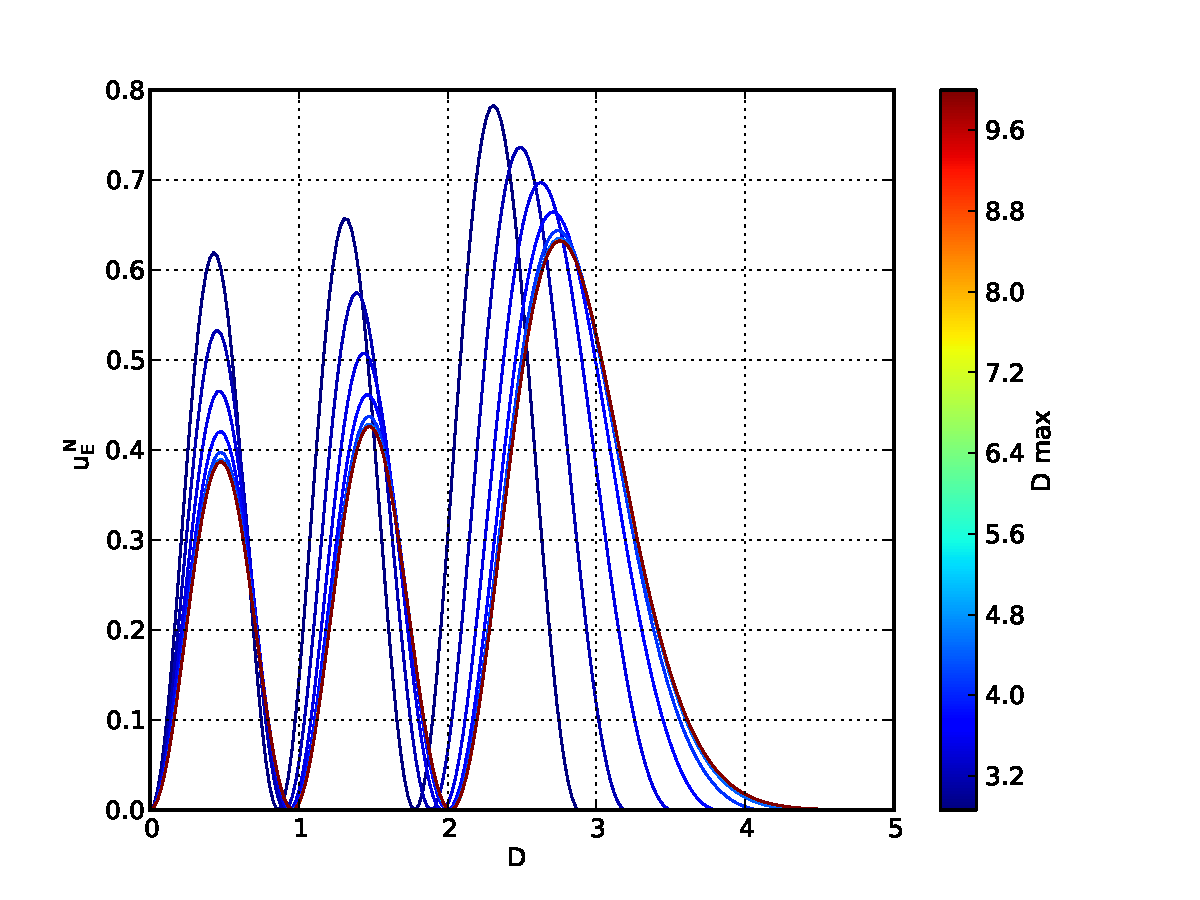
\includegraphics[width=0.81\linewidth]{rhoMaxAnalysis1.pdf}
    \caption{Convergence of the squared wavefunction for the first
        eigenstate of the harmonic oscillator as a function of $\rhomax$
    for $N=200$. The solutions have converged for $\rhomax > 4$.}
    \label{fig:rhoMax1}
\end{figure}

\begin{figure}[H]
    \centering
    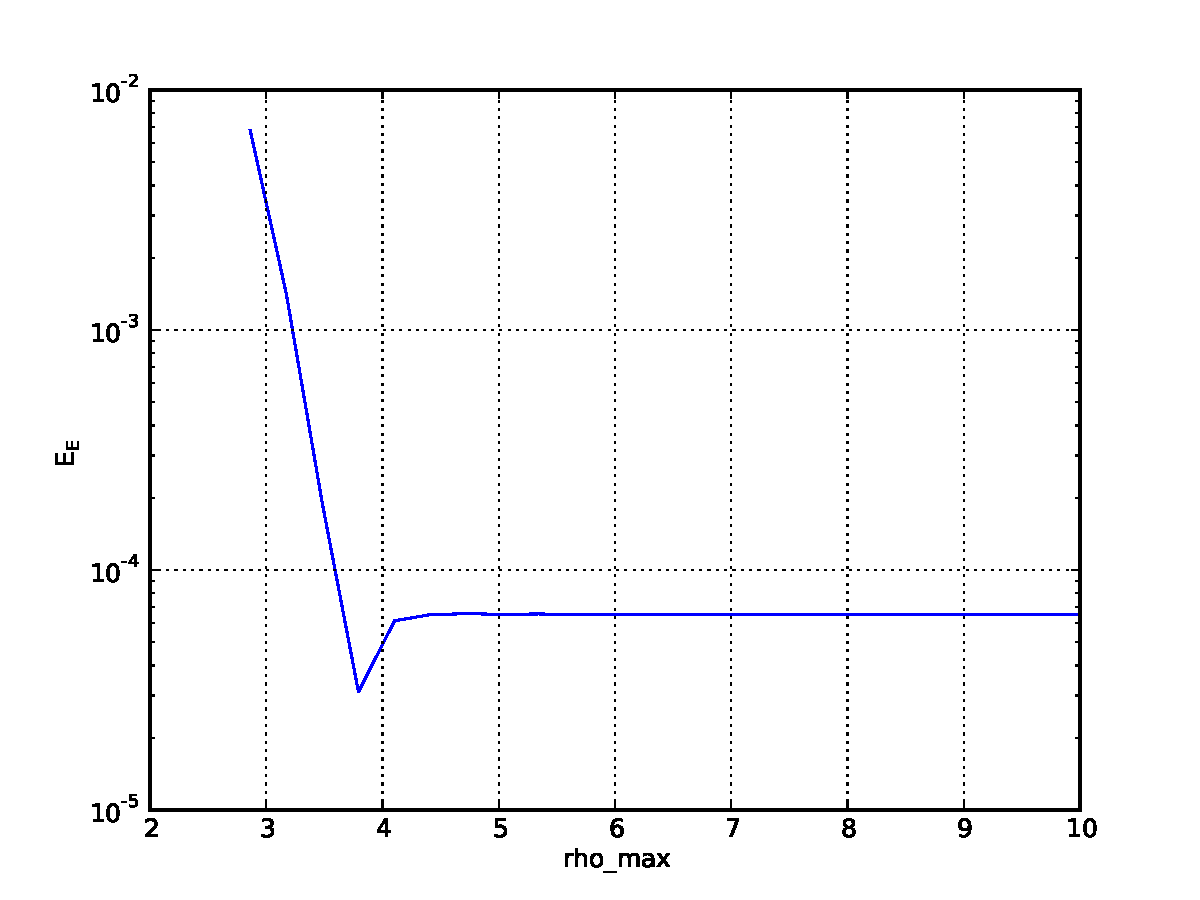
\includegraphics[width=0.81\linewidth]{rhoMaxAnalysis2.pdf}
    \caption{Convergence of the relative error of the first three
        eigenvalues of the 3D harmonic oscillator for increasing $\rhomax$,
        with constant step size $h$. For values above $\rhomax = 5$, no
    improvement is made.}
    \label{fig:rhoMax2}
\end{figure}


\begin{figure}[H]
    \centering
    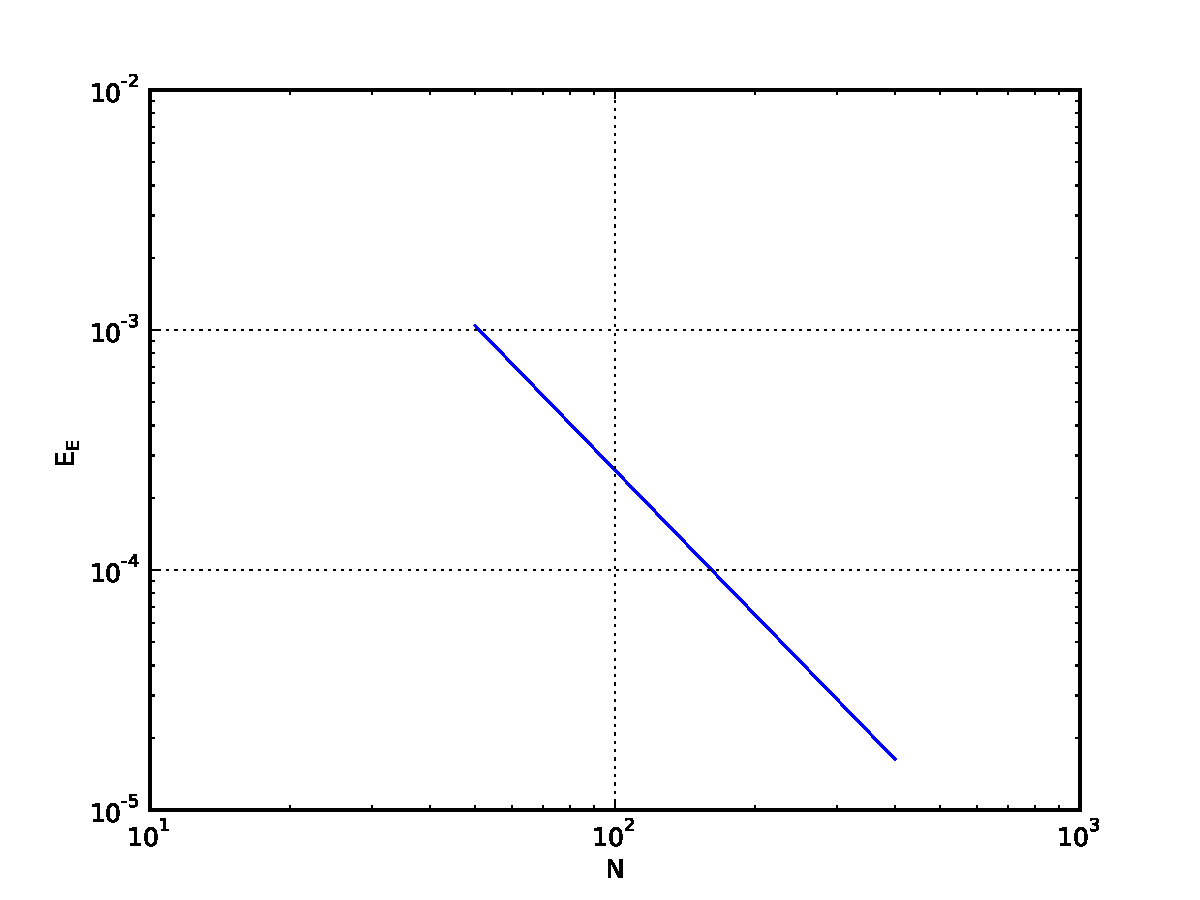
\includegraphics[width=0.85\linewidth]{dimAnalysis2.pdf}
    \caption{Relative error of the three first eigenvalues of the
    non-interacting harmonic oscillator as a function of $N$. $N=200$
produces relative error $\epsilon_i < 10^-4$ for all $i\in{1,2,3}$. The
average gradient of the three functions are $-1.81, -1.67$ and $ -1,60$
respectively.} 
    \label{fig:dim2}
\end{figure}

\subsubsection{Iterations}
Naively one can predict that the number of uses of the rotation algorithm
increases with the amount of matrix elements, $\bigO{N^2}$.
The results \Cref{fig:iterations} verifies this, showing a dependence of
$\bigO{N^{2.06}}$.



\begin{figure}[H]
    \centering
    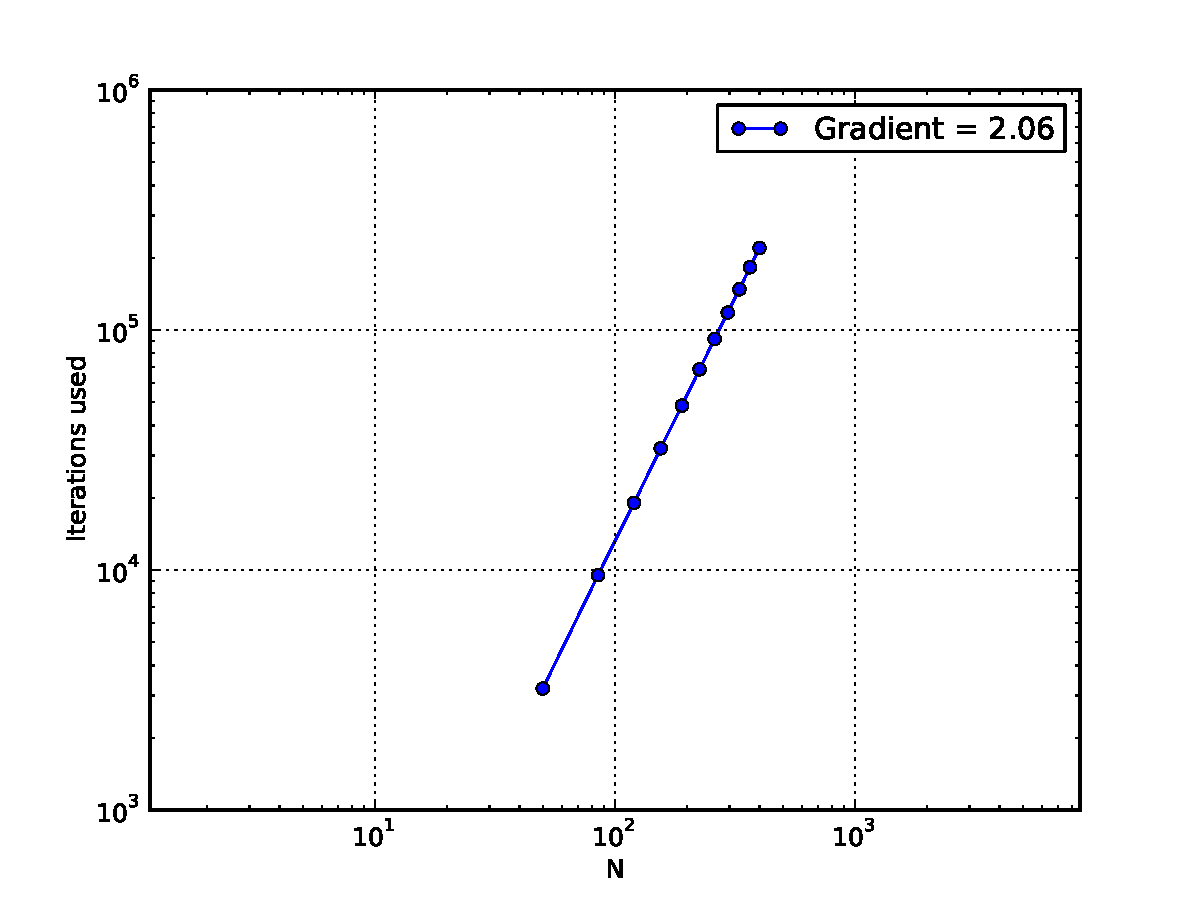
\includegraphics[width=0.83\linewidth]{iterations.pdf}
    \caption{Log-log plot of iterations of jacobi rotate used for the
        Jacobis method to produce a diagonalized (within a certain
        tolerance) matrix, as a function of $N$. The slope in the log plot
        is $2.06$, corresponding to a $\bigO{N^{2.06}}$ dependence.}
    \label{fig:iterations}
\end{figure}


\subsection{Interacting case}
The normalised wave function as a function of the relative coordinate between
electrons in the harmonic oscillator can be seen in \cref{fig:waveFunc}.
A larger value of $\omega_r$ causes a higher electron density. We got the
following three first eigenvalues for the electron:


\begin{center}
\begin{tabular}{ | c | c | c | c | }
    \hline
    $\omega_r$&$E_1$&$E_2$&$E_3$     \\
    $1/10$ & $0.106$ & $0.142$ & $0.178$ \\
    $1/4$ & $1.250$ & $2.190$ & $3.150$ \\
    $1/2$ & $2.230$ & $4.134$ & $6.074$ \\
    $1$ & $4.058$ & $7.909$ & $11.819$\\
    $5$ & $17.448$ & $37.070$ & $56.850$ \\
    \hline
 \end{tabular}
\end{center}




\begin{figure}[H]
    \centering
    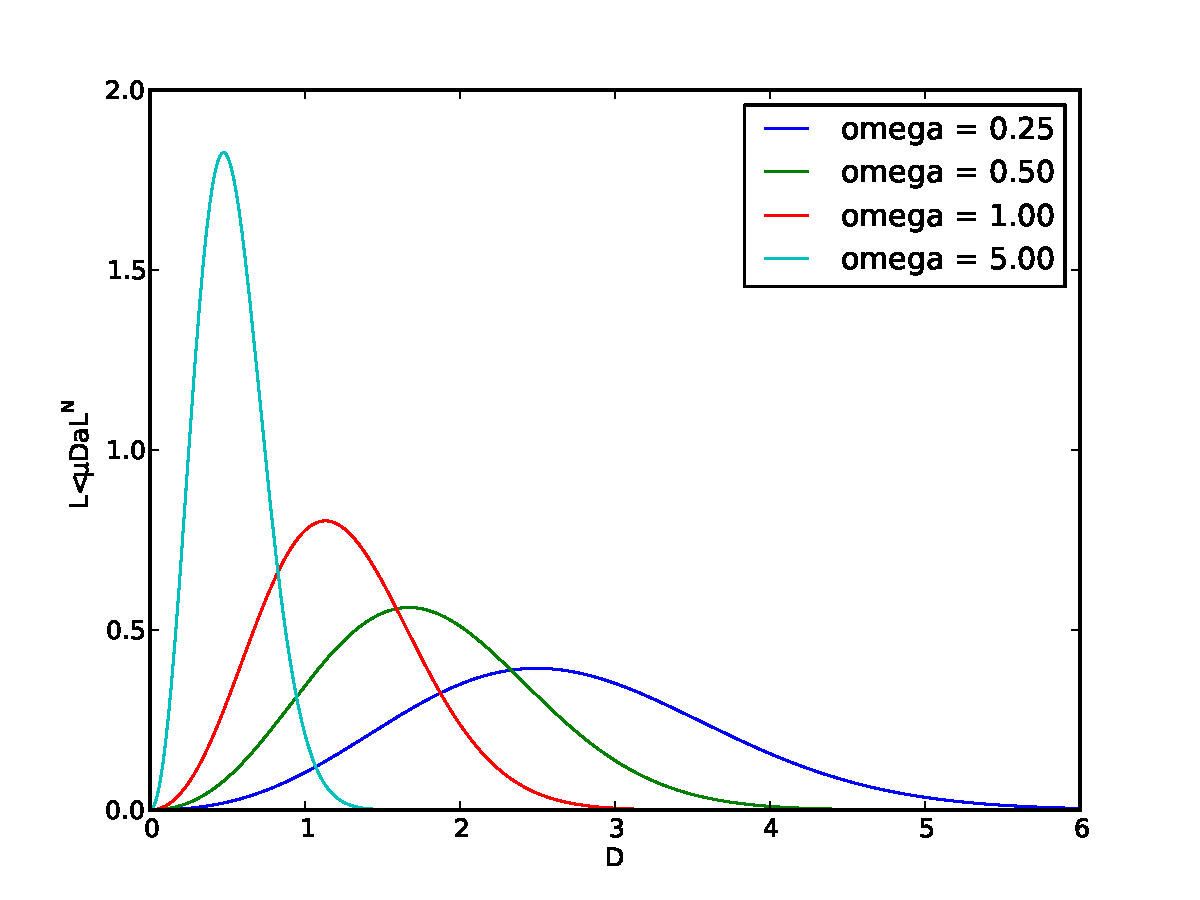
\includegraphics[width=0.85\linewidth]{waveFunc.pdf}
    \caption{The normalised wave functions of the relative coordinate for two
    interacting electrons, for the given $\omega_r$. The lowest value 
$\omega = 0.01$ stretched the wave function too much; it didn't even fit our
plot. One can see that the low energy bound states are spread out more for weak
potentials. }
    \label{fig:waveFunc}
\end{figure}



